\section{Što je konvolucija}
Konvolucija je u svojoj srži jednostavna matematička operacija koja je prikladna za obradu signala.
U osnovi, fotografija je vrsta signala, a konvolucija je crna kutija koja pretvara jedan signal, odnosno, sliku, u drugi.
Prednost konvolucije je što ne gleda samo jednu vrijednost, već i susjedne vrijednosti, pružajući tako dodatan kontekst.

\section{Jezgra konvolucije (\emph{eng. Kernel})}
Jezgra konvolucije, često nazvana \emph{prozor}, matrica je malih, neparnih dimenzija najčešće $3 \times 3$ ili $5 \times 5$.
Primjer jezgre može biti: 
$$
\begin{bmatrix}
	-1 & 0 & -1 \\
	-1 & 8 & -1 \\
	-1 & 0 & -1
\end{bmatrix}
$$
Jezgrom se prelazi preko željene matrice svim retcima i stupcima izvodeći u svakom koraku množenje po članovima (\cite{conv_pres}), primjerice:

\[
\begin{bmatrix}
	4 & 1 & 5\\
	1 & 2 & 6 \\
	9 & 7 & 3
\end{bmatrix}
\times
\begin{bmatrix}
	-1 & 0 & -1 \\
	-1 & 8 & -1 \\
	-1 & 0 & -1
\end{bmatrix}
=
\begin{bmatrix}
	-4 & 0 & -5\\
	-1 & 16 & -6 \\
	-9 & 0 & -3
\end{bmatrix}
\]
Jezgra konvolucije i sama konvolucija prikladni su za obradu slike iz razloga što računalo sliku i vidi kao dvodimenzionalnu matricu.
Spomenuto je lako zamislivo posebice u slučaju crno-bijele slike gdje vrijednosti mogu biti $\in [0, 255]$, gdje je $0$ crna, a $255$ bijela boja.

\subsection{Rubne vrijednosti}
Problem koji se može javiti jest kako se koristiti rubnim vrijednostima za potrebe korištenja u jezgri.
Na primjer, gornji lijevi rub slike nema susjedne vrijednosti gore i lijevo od sebe.

\paragraph{Produljivanje}
u slučaju nedostatka susjedne vrijednosti na njegovo mjesto samo kopira najbližu postojeću vrijednost (Ilustracija \ref{fig:extend_edge}).

\paragraph{Obgrljivanje}
promatra sliku kao da je beskonačna po veličini, u obje osi.
U slučaju nedostatka vrijednosti  jednostavno dobiva vrijednost sa suprotne strane.
Također, to je metoda koju sam ja koristio u implementaciji i eksperimentima te pruža dobre rezultate (Ilustracija \ref{fig:wrap_edge}).

\paragraph{Preskakivanje}
uopće ne promatra rubne vrijednosti slike te zaobilazi problem nepostojećih rubnih vrijednosti u potpunosti.
Problem koji se može javiti jest da je rezultantna matrica $G$ manja od izvorne matrice $F$.

\begin{figure}
	\caption{Grafički prikaz dva različita načina upravljanja rubnim vrijednostima s označenim rubom slike i trenutnom pozicijom jezgre}
	\begin{subfigure}[t]{0.48\textwidth}
		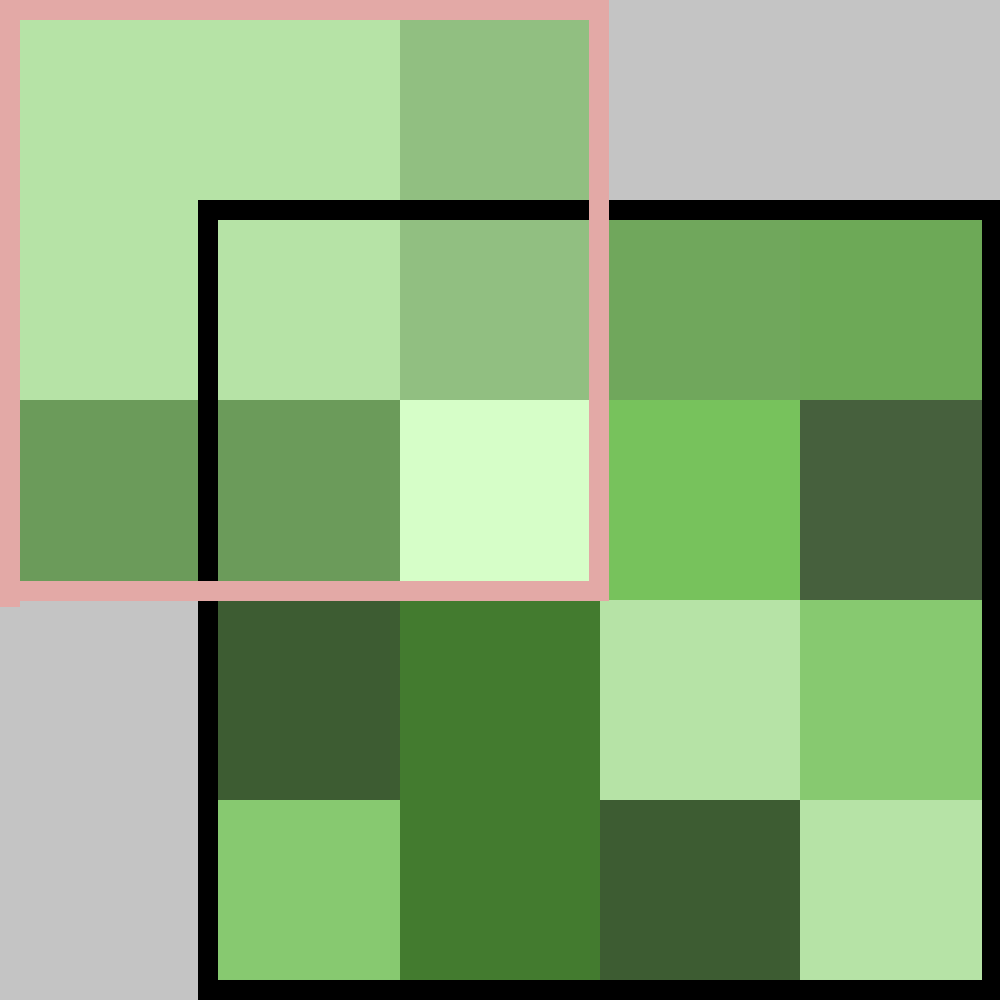
\includegraphics[width=\textwidth]{Illustrations/extend.png}
		\caption{Upravljanje rubom produljivanjem trenutno promatrane jezgre}
		\label{fig:extend_edge}
	\end{subfigure}
	\begin{subfigure}[t]{0.48\textwidth}
		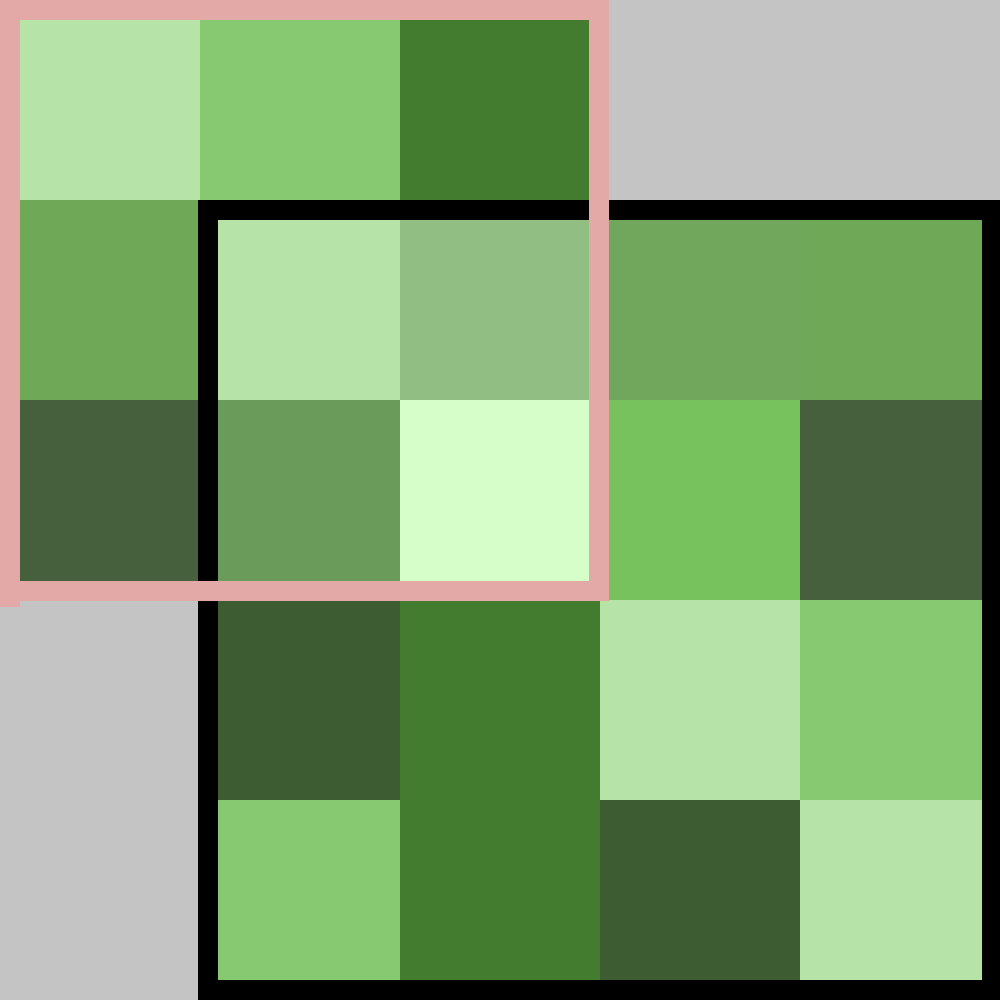
\includegraphics[width=\textwidth]{Illustrations/wrap.png}
		\caption{Upravljanje rubom obgrljivanjem slike}
		\label{fig:wrap_edge}
	\end{subfigure}
\end{figure}

\section{Operacija konvolucije}
Konvolucija se matematički može prikazati kao
$$g(x, y) = \omega \cdot f(x,y) = \sum_{dx=-a}^{a} \sum_{dy=-b}^{b} \omega(dx, dy)\cdot f(x + dx, y + dy)$$
gdje je $g(x,y)$ rezultantna slika, $f(x, y)$ izvorna slika a $\omega$ jezgra.

\section{Provedeni eksperimenti}

\subsection{Micanje šuma}
Prvi problem koji sam definirao je problem rekonstrukcije slike s dodanim šumom.
Promatramo sliku, definiranu kao matrica $I$ veličine $w \times h$ gdje za svaki element $x$ na koordinatama $(i, j)$ vrijedi $x_{(i, j)} \in [0, 255]$ što predstavlja intentzitet boje od crne prema bijeloj. \\
Sintetički šum koji sam dodao vrste \emph{"Salt and pepper"} odnosno soli i papra nazvan je tako jer određeni postotak nasumičnih vrijednosti postavi na bijelu ili crnu boju (slika \ref{fig:salt_pepper_example}).

\begin{figure}
	\centering
	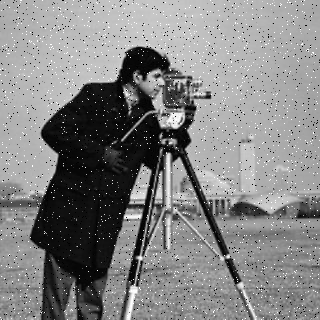
\includegraphics[width=0.5\linewidth]{Experiments/GrainRemoval/input_example.png}
	\caption{Primjerak fotografije s $5\%$ šuma soli i papra}
	\label{fig:salt_pepper_example}
\end{figure}

Postotak slike na koji sam odlučio primjeniti šum je $5\%$, slično kao i \cite{cgp_image_processing} i \cite{Sekanina2011}.
U nastavku rada također ću predstaviti rezultate na većem postotku šuma od $40\%$.

Cilj eksperimenta je evoluirati filter $f(x)$ koristeći konvolucijske metode i CGP koji će od oštećene slike $D$ reproducirati novu $Y = f(D)$ što bližu neoštećenom originalu $I$.
$$
\min_{Y, i, j} |Y_{(i, j)} - I_{(i, j)}|
$$
Iz susjedstva svake vrijednosti želimo dobiti što precizniju promatranu vrijednost. \\
Polazišna pretpostavka je ta su susjedne vrijednosti na slici u međusobnoj korelaciji do određene mjere te mogu pomoći u zaključivanju originalne vrijednosti.
Problem koji se može javiti je da u promatranom susjedstvu također imamo vrijednost koja je šum što narušava pretpostavku korelacije.
Navedeni problem je zanemaren te je CGP-u ostavljeno kao problem koji treba riješiti bez ljudskog znanja.

Jezgra $\omega$ koju sam odlučio koristiti je veličine $3 \times 3$ koja promatra $Moore$-ovo susjedstvo (\cite{jakobovic}).

\[
	\omega_{(i, j)}
	=
	\begin{bmatrix}
		x_{(i - 1, j - 1)} && x_{(i - 1, j)} && x_{(i - 1, j + 1)}\\
		x_{(i, j - 1)} && && x_{(i, j + 1)}\\
		x_{(i + 1, j - 1)} && x_{(i + 1, j)} && x_{(i + 1, j + 1)}
	\end{bmatrix}
\]
Razmišljanje iza korištenja jezgre koja ne koristi središnju, promatranu vrijednost je što tu vrijednost upravo pokušavamo predvidjeti i njena vrijednost, posebice ako je šum ne smije imati utjecaja.
Detaljniji prikaz djelovanja i rezultata mooreove jezgre vidljiv je na ilustraciji \ref{fig:moore_example}

\begin{figure}
	\centering
	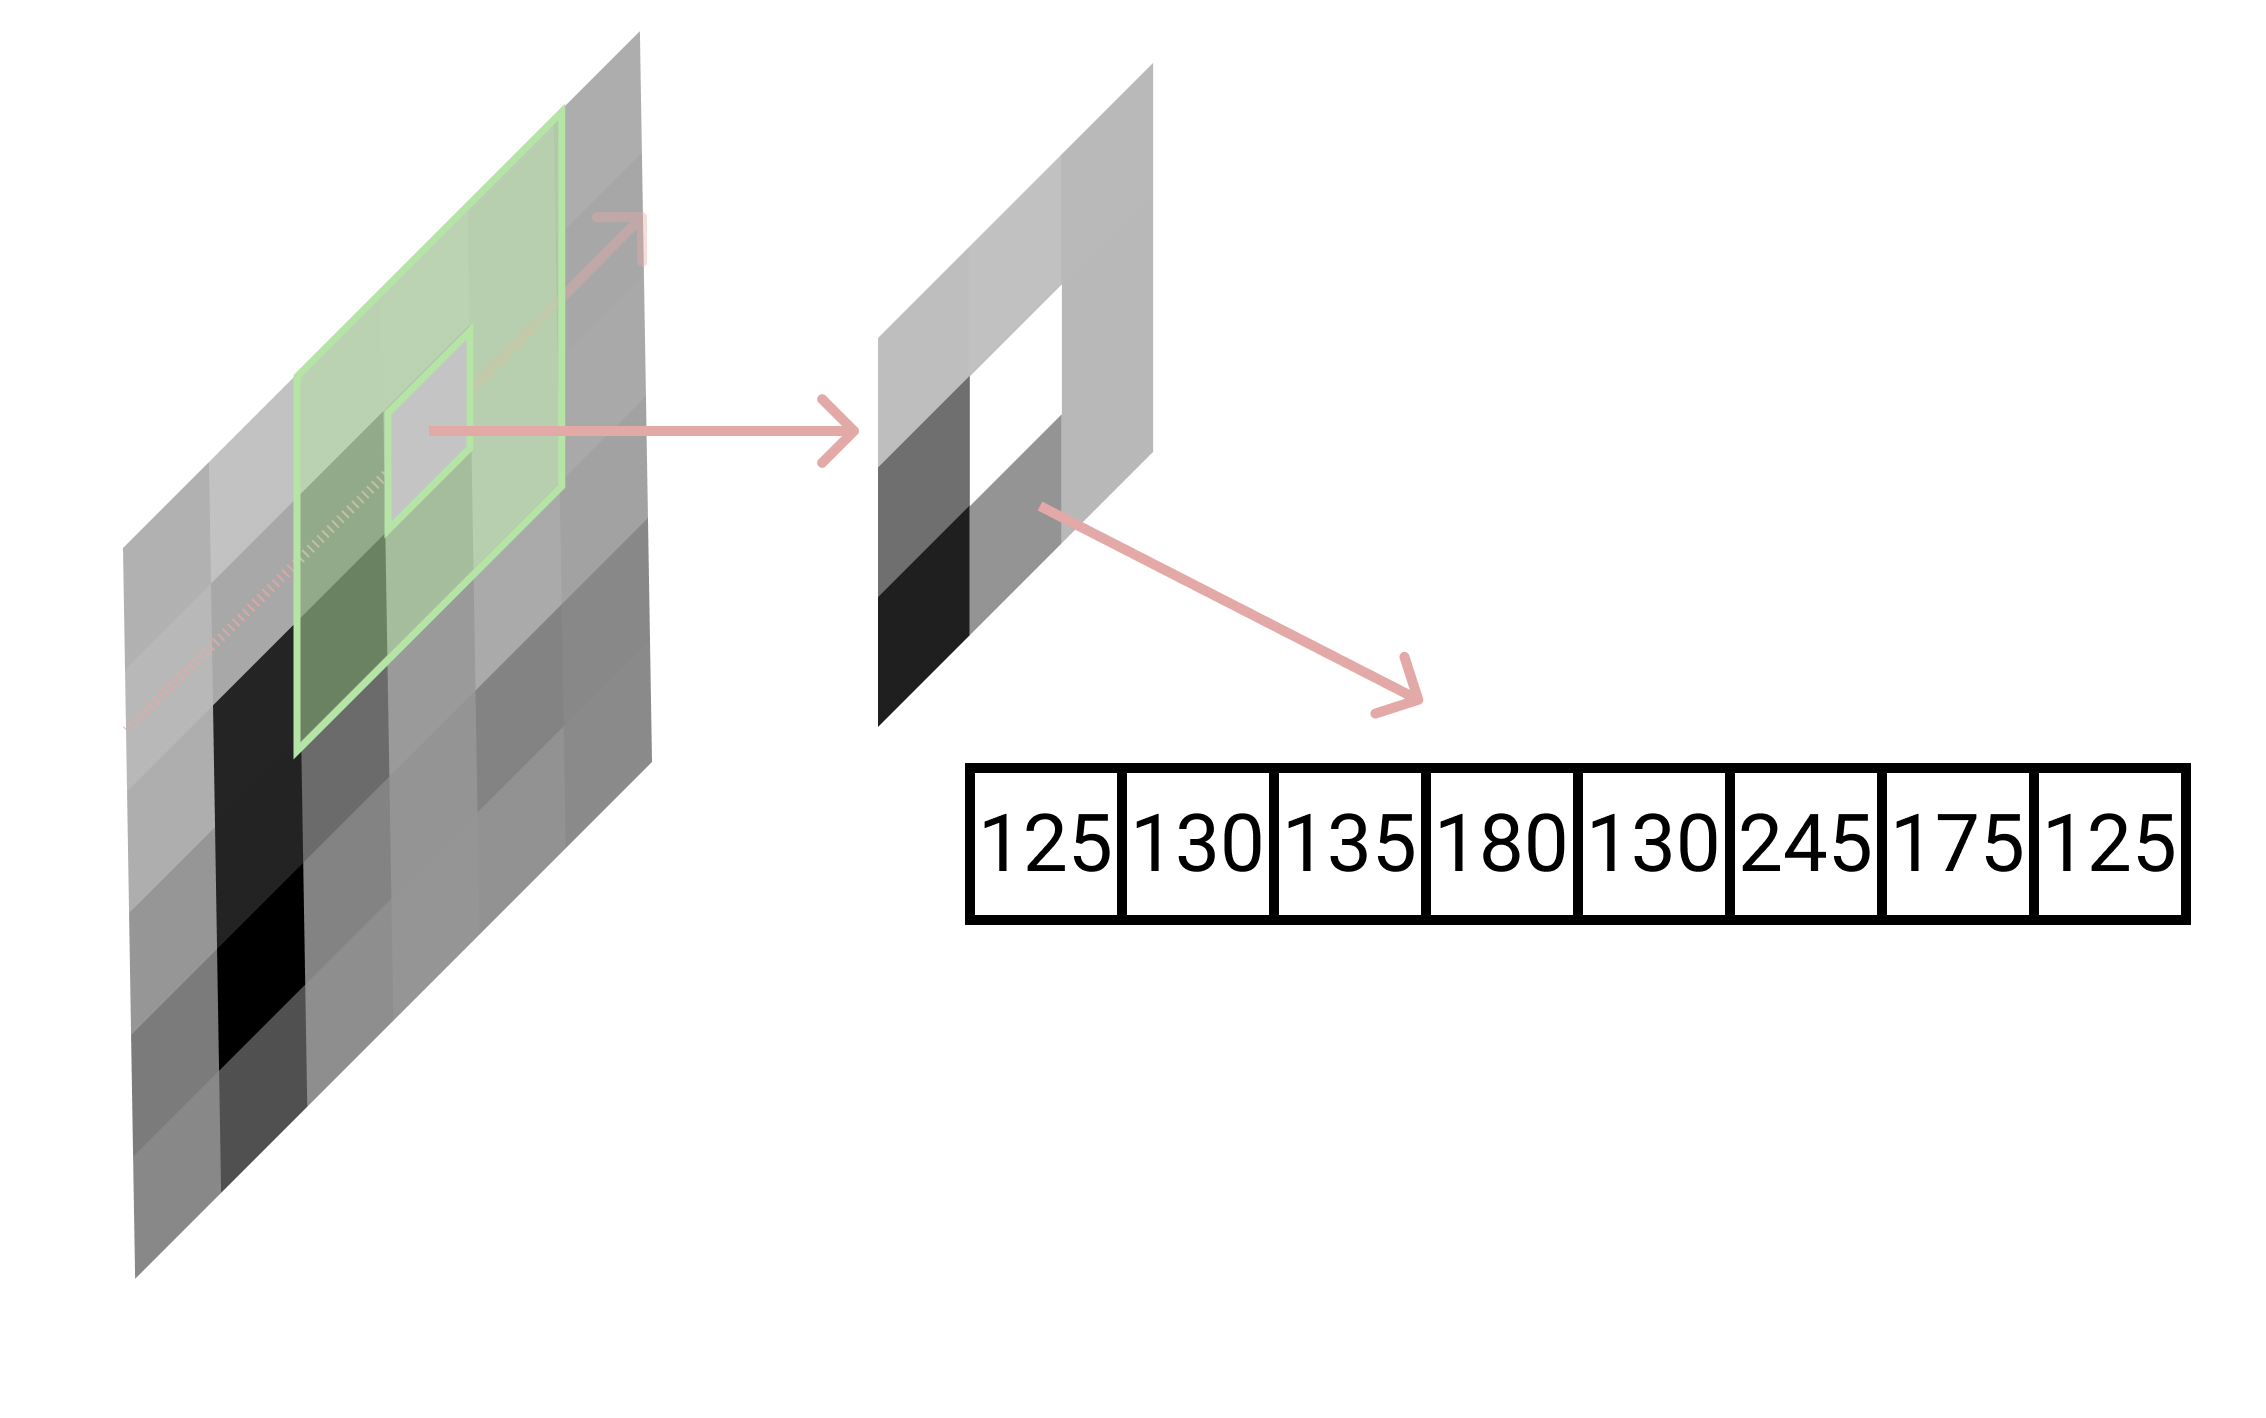
\includegraphics[width=0.8\linewidth]{Illustrations/moore.png}
	\caption{Primjer čitanja slike mooreovom jezgrom te transformacija iz preuzetog dijela slike u vektor vrijednosti koristivih CGP-u}
	\label{fig:moore_example}
\end{figure}



\subsection{Detektiranje rubova (\emph{eng. Edge detection})}
Detektiranje rubova može se promatrati kao tehnika čitanja rubova objekata vidljivih na slici.
Samo po sebi jedna je od osnovnih, nisko razinskih tehnika računalnog vida s mnogim primjenama visoke razine, uključujući detekciju objekata i segmentaciju slike (\emph{eng. Image Segmentation}) (\cite{Liu_2019}).

Problem je definiran kao pokušaj imitiranja rada \emph{Sobel} operatora.

 \paragraph{Sobel operator} također je operator koji koristi konvoluciju.
 Koriste se dvije konvolucijske jezgre (\cite{Sekanina2011}):
 \[
	 p = \frac{1}{8}
	 \begin{bmatrix}
		 -1 && 0 && 1 \\
		 -2 && 0 && 2 \\
		 -1 && 0 && 1
	 \end{bmatrix}
	 ,\ 
	 q = \frac{1}{8}
	 \begin{bmatrix}
		 -1 && -2 && -1 \\
		 0 && 0 && 0 \\
		 1 && 2 && 1
	 \end{bmatrix}
 \]
Zajedno, jezgre služe kako bi se izračunao gradijent slike.
Jezgra $p$ koristi se kako bi se izračunala procjena derivacije za horizontalne promjene, a $q$ za vertikalne. \\
Vrijednost novonastale slike $G$ na koordinatima $(i, j)$ računa se kao
$$
G_{(i, j)} = c + |p_{(i, j)}| + |q_{(i, j)}|
$$
gdje je $c$ proizvoljna konstanta, npr. $c = 128$.
Primjer djelovanja Sobel operatora na fotografiju Lene vidljiv je na slici \ref{fig:lena_sobel}.

\begin{figure}
	\centering
	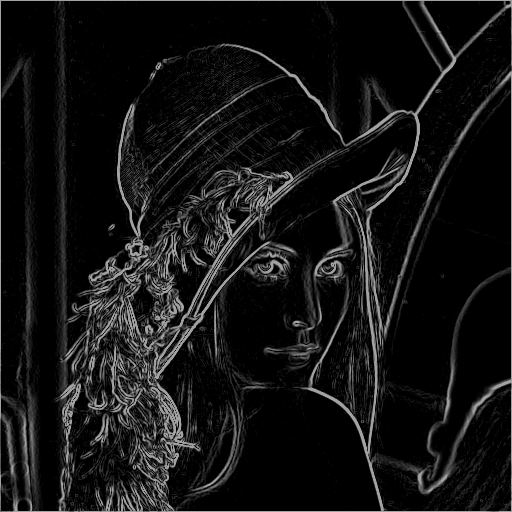
\includegraphics[width=0.6\linewidth]{Experiments/EdgeDetection/lena_sobel.png}
	\caption{Primjer djelovanja Sobel operatora na fotografiju Lene}
	\label{fig:lena_sobel}
\end{figure}

\subsubsection{Postavke}
Za razliku od micanja šuma koristi se konvolucijska jezgra koja prihvaća i srednju promatranu vrijednost.
Time, filter možemo definirati kao $f(x): [0, 255]^9 \rightarrow [0, 255]$.

Fotografije koje su se promatrale u trening i validacijskoj fazi vidljive su na slici \ref{fig:edge_detection_train_val_in}.
Umjesto direktne usporedbe sa Sobel slikama, odlučio sam se na usporedbu sa slikama dobivenim \emph{Canny} algoritmom.
Slike nastale primjenom Canny algoritma imaju vrijednosti $0$ ili $1$ ovisno pripada li promatrana vrijednost na koordinatama $(i, j)$ rubu što sam koristio kao prednost u razvoju modela.
Jednako kao u više-kategoričkoj klasifikaciji gdje se koristi vektor vrijednosti gdje su sve vrijednosti $0$ osim točne koja je $1$ (\emph{eng. One Hot Encoding}).

\begin{figure}
	\centering
	\caption{Fotografije Lene i Kamermana nakon primjene detekcije ruba \emph{Canny} algoritmom}
	\begin{subfigure}[t]{0.45\textwidth}
		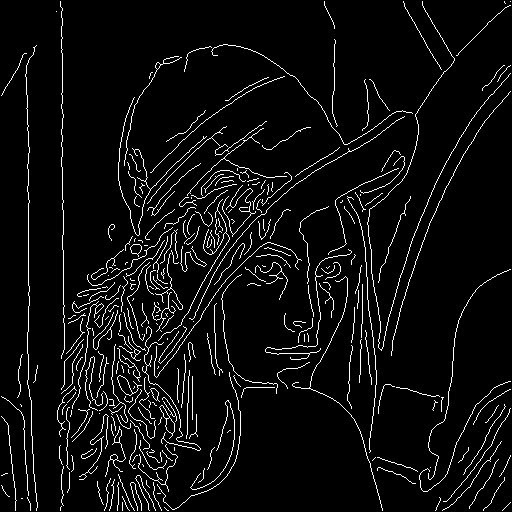
\includegraphics[width=\textwidth]{Experiments/EdgeDetection/lena_canny.jpg}
		\caption{Lena nakon primjene Canny filtera}
		\label{fig:lena_canny}
	\end{subfigure}
	\begin{subfigure}[t]{0.45\textwidth}
		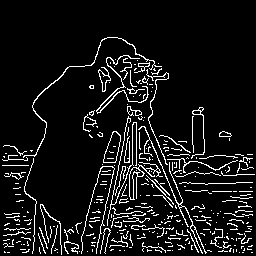
\includegraphics[width=\textwidth]{Experiments/EdgeDetection/cameraman_canny.jpg}
		\caption{Kamerman nakon primjene Canny filtera}
		\label{fig:camerman_canny}
	\end{subfigure}
	\label{fig:edge_detection_train_val_in}
\end{figure}

Problem koji se rano javio je što je $\approx 70\%$ slike vrijednosti $0$, odnosno, crno.
Rezultat toga i korištenja $L1$ pogreške je navođenje modela da teži samo predviđanju te vrijednosti.
Korištenje srednje kvadratne pogreške (\emph{eng. Mean Squared Error (MSE)})
$$err = \frac{1}{n}\sum_{i=1}^{n}(y_{cgp} - y_{skup\ podataka})^2$$
pokazalo se dobrim rješenjem.
U slučaju veće razlike npr. predviđanje $1$ na željenu vrijednost $0$ unutar sume rezultiralo bi razlikom od $255^2$, dok bi manje razlike težile ka $0$.

Tablica \ref{table:edge_detection_function_set} prikazuje funkcije koje su se mogle koristiti u čvorovima.
Vrijednosti nisu morale biti unutar skupa $[0, 255]$, a na izlazu bi se prilagodile najbližoj rubnoj vrijednosti u slučaju da izlaz nije unutar skupa.
Također, ako se funkciji $3$, dijeljenju, prosljedi nepodržana vrijednost u nazivnik, funkcija se koristi kao funkcija identiteta, odnosno $f(x, y) = x$.
Algoritam odabira je $1 + \lambda$ s $\lambda = 8$.
Povećanje parametra $\lambda$ zahtjeva smanjenje najvećeg dozvoljenog broja iteracija koji je postavljen na $20$, puno manje nego pri micanju šuma gdje je definirano kao $500$.

\begin{table}
	\centering
	\begin{tabular}{||c c c c||}
		\hline
		Adresa funkcije & Funkcija & Broj ulaza & Broj izlaza\\ [0.5ex]
		\hline \hline
		0 & $x + y$ & 2 & 1\\
		1 & $x - y$ & 2 & 1\\
		2 & $x \cdot y$ & 2 & 1\\
		3 & $\frac{x}{y}$ & 2 & 1 \\
		4 & $\sqrt{x}$ & 1 & 1\\
		5 & $avg$ & 9 & 1\\
		6 & $min$ & 9 & 1\\
		7 & $max$ & 9 & 1\\
		8 & $\ln(x)$ & 1 & 1\\
		9 & $\sin(x)$ & 1 & 1\\
		10 & $\cos(x)$ & 1 & 1\\
		11 & $step(x)$ & 1 & 1\\ [1ex]
		\hline
	\end{tabular}
	\caption{Funkcije korištene pri detekciji rubova}
	\label{table:edge_detection_function_set}
\end{table}

Promatrani podskupovi veličina su $40 \times 40$.
Time, skup podataka sastoji se od $1600$ vektora ($|v| = 9$), po jedan za svaku promatranu konvolucijsku jezgru.
Trening i validacijski skup uzet je sa iste fotografije Lene u dva odvojena podskupa (\ref{fig:edge_detection_in_out_pair_example}), dok je za testnu fotografiju odabrana fotografija kamermana.

\begin{figure}
	\centering
	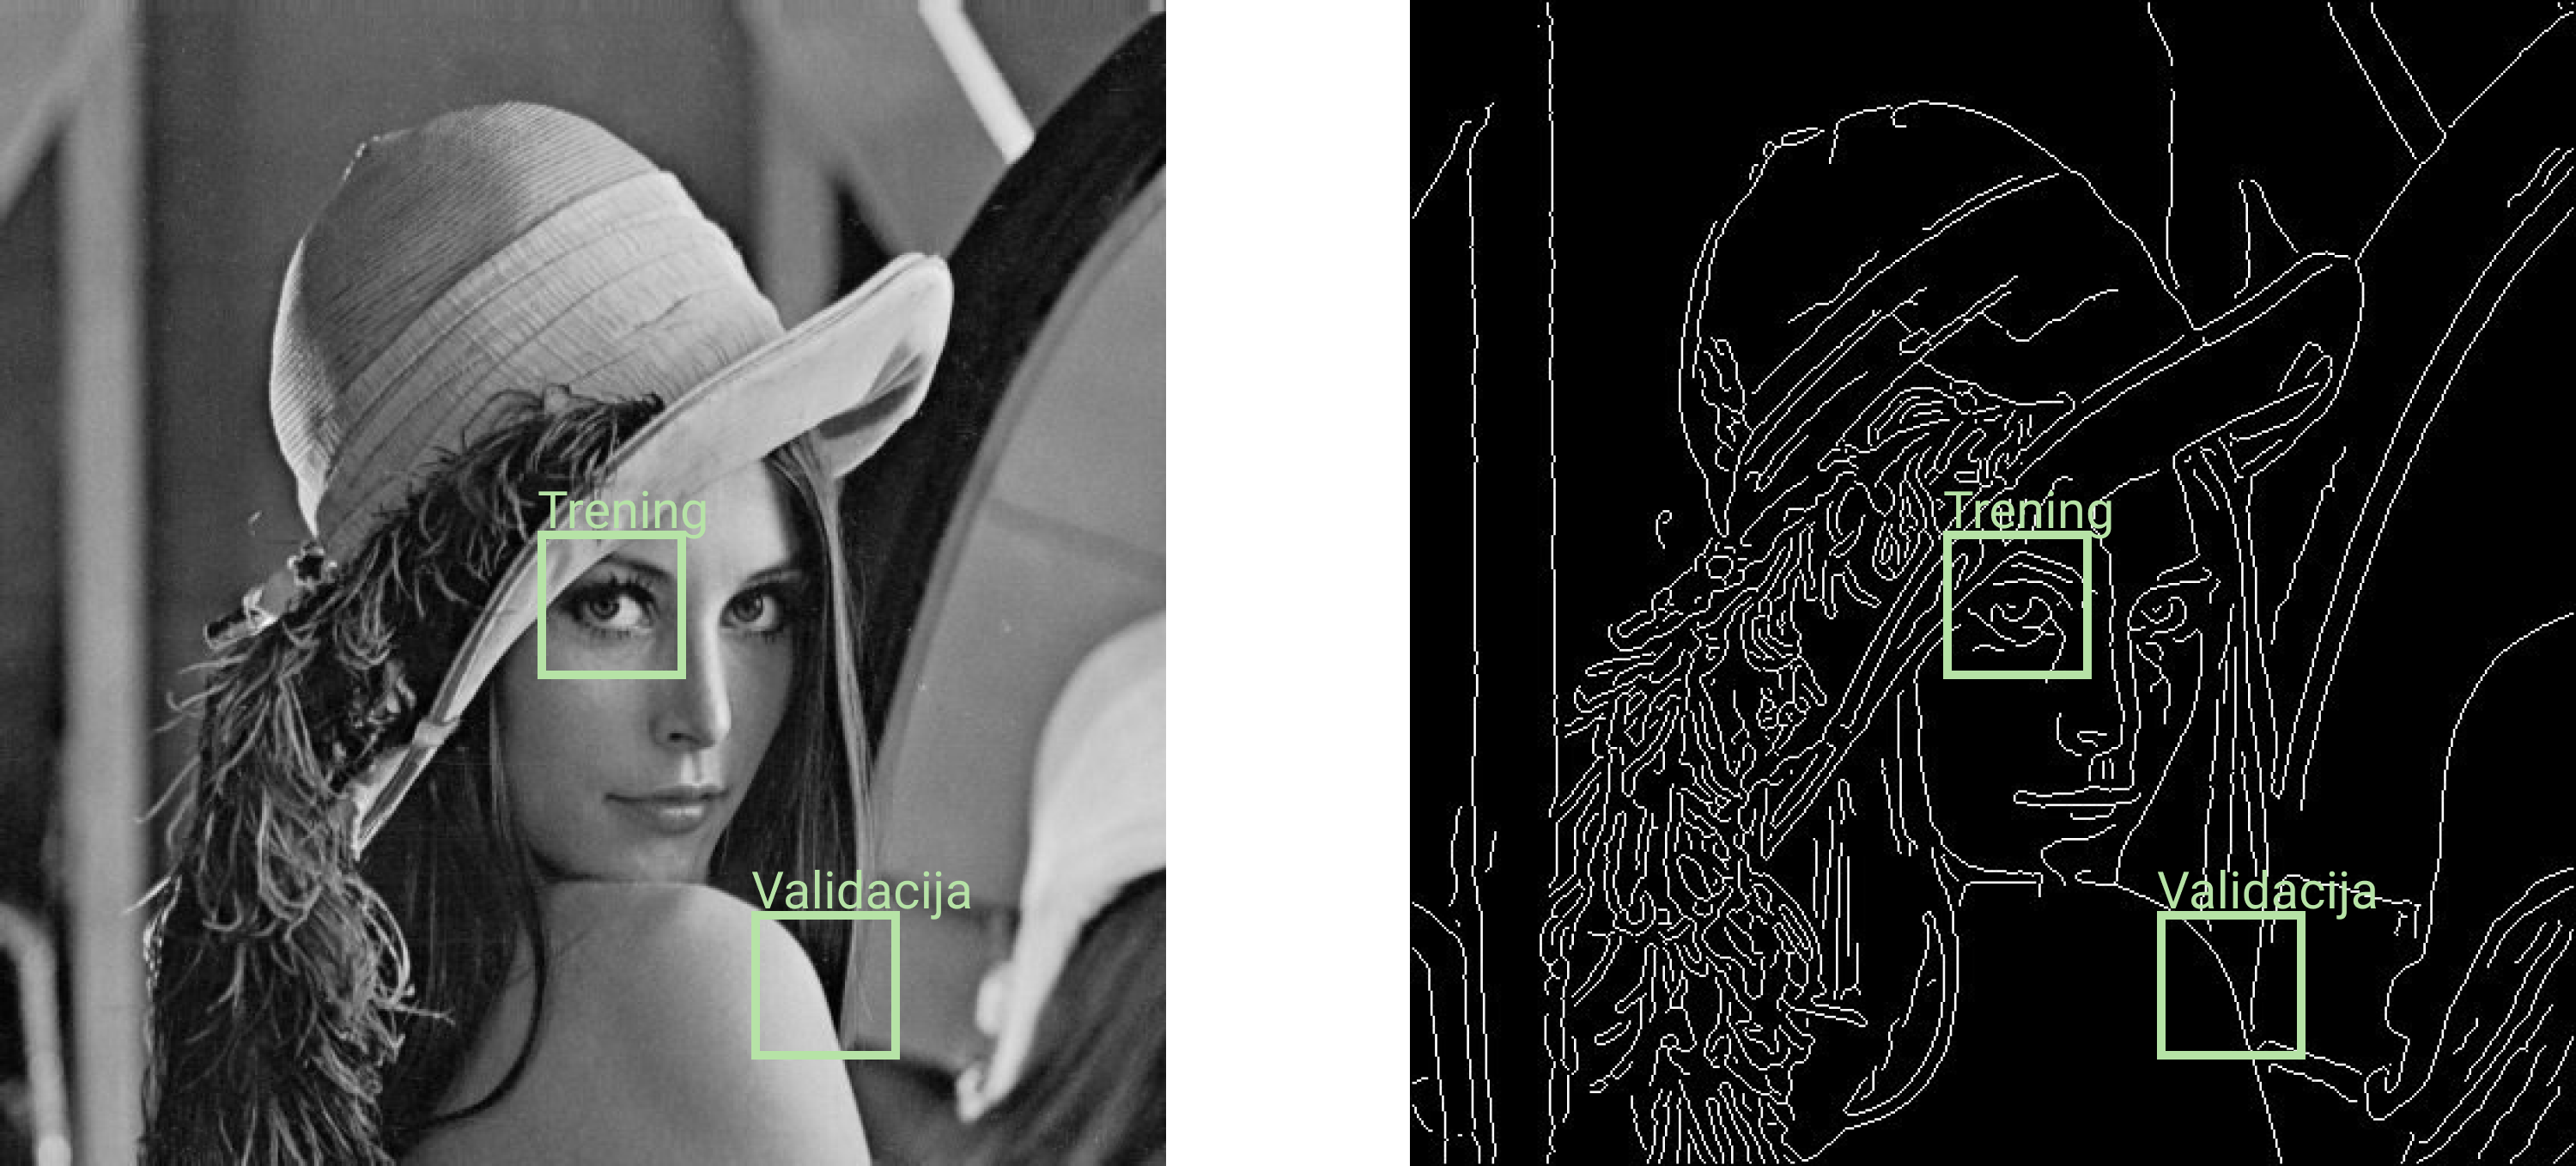
\includegraphics[width=\linewidth]{Experiments/EdgeDetection/edge_detection_in_out_pair.png}
	\caption{Ulazna i željena izlazna slika za detekciju ruba s označenim podskupovima za trening i validaciju}
	\label{fig:edge_detection_in_out_pair_example}
\end{figure}

\subsubsection{Rezultati}
Rezultati detekcije ruba vidljivi su na slikama \ref{fig:edge_detection_results}. % TODO: Dodati graf!
Pomalo neočekivano, rezultati izgledaju bolje na testnoj slici, no to pridodajem značajkama fotografije pogodnijim za detekciju rubova.
Zbog toga, vjerujem da je dosta težak zadatak za detekciju rubova fotografija s vidljivom kosom ili bilo kakvim sitnim detaljima.
Veliku ulogu igrao je i izbor podskupa iz kojeg se isčitavaju podaci za trening.
Količina praznog dijela, vrsta i broj vidljivih krivulja, zajedno s ispravnim odabirom funkcije koju minimiziramo igra najveću ulogu.
U usporedbi s problemom micanja šuma, detekcija rubova rješenje pronalazi iznimno brzo.
Svako pokretanje koje je završilo s uspješnim pronalaskom rješenja konvergiralo je u $\leq 10$ iteracija.

\begin{figure}
	\centering
	\caption{Fotografije Lene i Kamermana prije i nakon detekcije rubova}
	\begin{subfigure}[t]{0.48\textwidth}
		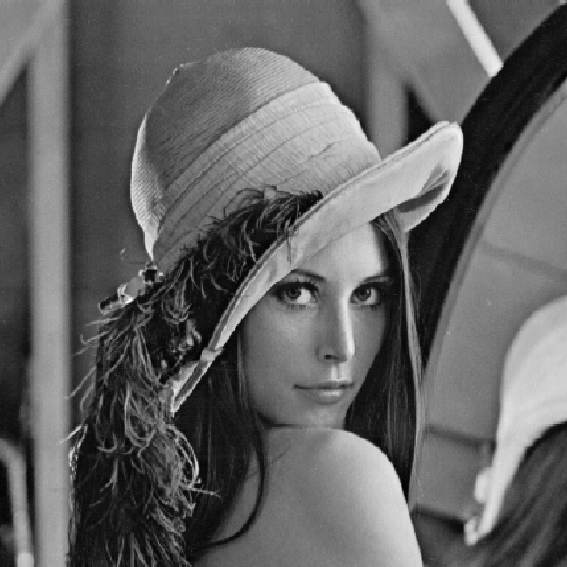
\includegraphics[width=\textwidth]{Experiments/GrainRemoval/lena.png}
	\end{subfigure}
	\begin{subfigure}[t]{0.48\textwidth}
		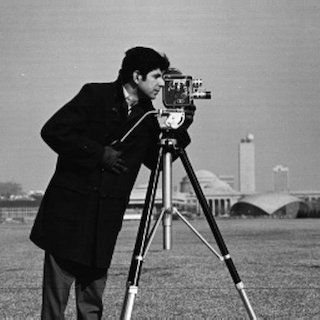
\includegraphics[width=\textwidth]{Experiments/GrainRemoval/cameraman.jpg}
	\end{subfigure}
	\begin{subfigure}[t]{0.48\textwidth}
		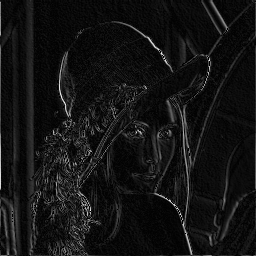
\includegraphics[width=\textwidth]{Experiments/EdgeDetection/lena_edges.png}
	\end{subfigure}
	\begin{subfigure}[t]{0.48\textwidth}
		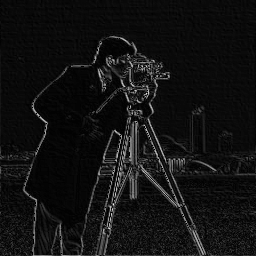
\includegraphics[width=\textwidth]{Experiments/EdgeDetection/camerman_edges.png}
	\end{subfigure}
	\label{fig:edge_detection_results}
\end{figure}

Graf \ref{fig:edge_detection_graph} pokazuje kretanje pogreške na trening i validacijskom skupu podataka.
Greška se čini niska već pri pokretanju no to je zbog prirode algoritma.
Iz početnog stvaranja potencijalnog roditelja kao najbolji odabire se najčešće onaj koji veliku večinu rezultata računa kao $0$ što je u svakom slučaju točno za većinu skupa podataka.
Daljni koraci vrlo brzo konvergiraju točnijim rješenjima.

\begin{figure}
	\centering
	\caption{\emph{MSE} pogreška na trening i validacijskom skupu kroz iteracije algoritma}
	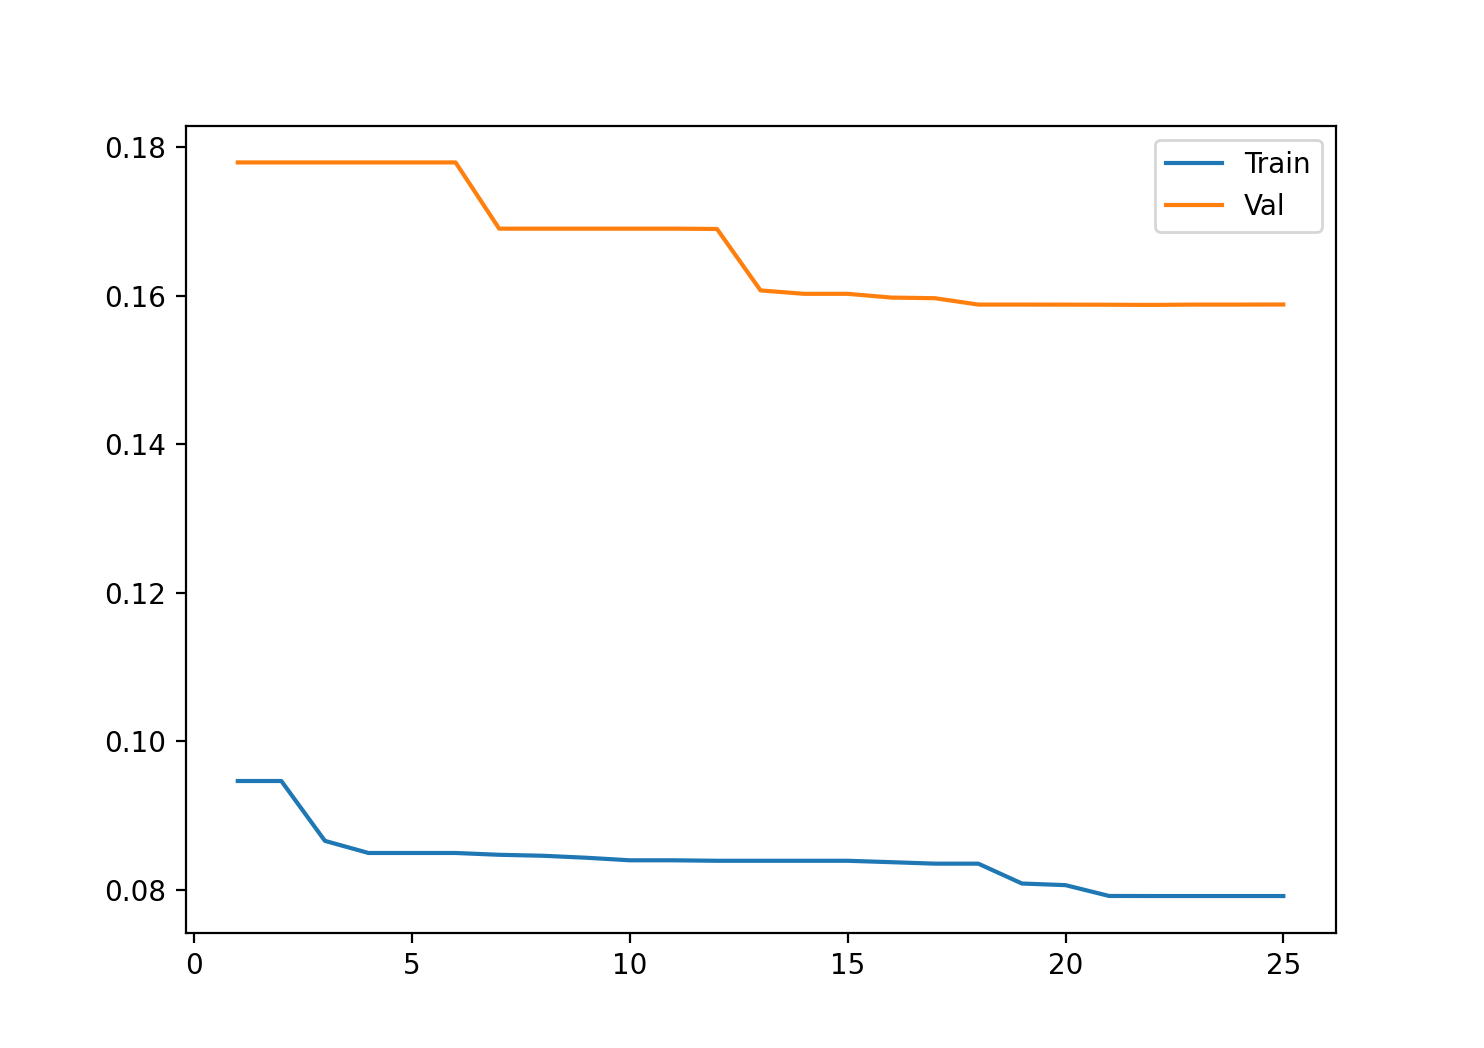
\includegraphics[width=0.6\linewidth]{Experiments/EdgeDetection/edge_detection_graph.png}
	\label{fig:edge_detection_graph}
\end{figure}

Tablica \ref{table:edge_detection_function_quality} prikazuje korisnost pojedinih funkcija.
Kao i u slučaju micanja šuma, svako mjerenje izvršeno je 10 puta te je uzet medijan kao vrijednost za izračun.
Vidljivo je da u ovom slučaju funkcije $step$, $sin$, $cos$ i $min$ ne doprinose radu algoritma, dok su se na primjer $ln$ i $avg$ pokazali važnim.
Zanimljiva je i usporedba funkcija $max$ i $min$ gdje je jedna doprinjela, a druga odmogla radu algoritma.

\begin{table}
	\centering
	\begin{tabular}{||c c||}
		\hline
		Izbačena funkcija & Utjecaj na pogrešku (manje je bolje)\\ [0.5ex]
		\hline \hline
		$step$ & $0.9065$\\
		$sin$ & $0.9100$\\
		$cos$ & $0.9685$\\
		$min$ & $0.9971$\\
		$\bm{osnova}$ & $\bm{1.0}$\\
		$x + y$ & $1.0063$\\
		$x \dot y$ & $1.0619$\\
		$x - y$ & $1.0711$\\
		$\frac{x}{y}$ & $1.2017$\\
		$max$ & $1.3360$\\
		$\sqrt{x}$ & $1.5425$\\
		$ln(x)$ & $1.5605$\\
		$avg$ & $1.5821$\\ [1ex]
		\hline
	\end{tabular}
	\caption{Analiza doprinosa pojedinih funkcija pri detekciji rubova. Osnovno mjerenje dozvoljava sve funkcije iz skupa.}
	\label{table:edge_detection_function_quality}
\end{table}

